\section{Theoretical Properties}
\label{sec:properties}

We collect the properties that make the ability tilt a principled allocator
rather than a heuristic. Throughout, the abilities $a$ are fixed and we view the
weights as the winning-probability map $w(C)$.

\begin{proposition}[Feasibility]
\label{prop:feasible}
For every positive-definite $C$ and every $a$, the weights lie in the
probability simplex: $w_i \ge 0$ and $\sum_i w_i = 1$.
\end{proposition}
\begin{proof}
Each realization contributes one unit of weight, divided evenly among the assets
attaining the minimum; summing over realizations leaves $w_i \ge 0$ with
$\sum_i w_i = 1$. (Even division, rather than a random award among the tied, is
also what keeps the estimator low-variance.)
\end{proof}
\noindent Long-only and fully-invested portfolios thus come for free---no
constraints, penalties, or projection onto the simplex.

\begin{proposition}[Index reproduction]
\label{prop:fixedpoint}
If the tilt correlation equals the calibration correlation,
$C_{\mathrm{tilt}} = C_{\mathrm{calib}}$, then $w = w^{\mathrm{target}}$.
\end{proposition}
\begin{proof}
The abilities are calibrated so that the race under $C_{\mathrm{calib}}$
reproduces the target; evaluating at $C_{\mathrm{tilt}} = C_{\mathrm{calib}}$
returns it.
\end{proof}
\noindent The tilt is therefore a \emph{controlled perturbation} of the
benchmark: the deviation is driven by $C_{\mathrm{tilt}} - C_{\mathrm{calib}}$
and bounded by the Lipschitz estimate of \Cref{thm:smooth}.

\begin{proposition}[Redundancy consistency]
\label{prop:redundancy}
Replace asset $k$ by two perfect duplicates $k', k''$ (equal ability, unit
variance, mutual correlation $1$, and the same correlation as $k$ with every
other asset). Then, splitting ties evenly,
\begin{equation*}
  w_{k'} + w_{k''} = w_k^{\setminus}, \qquad
  w_{k'} = w_{k''} = \tfrac12 w_k^{\setminus}, \qquad
  w_j = w_j^{\setminus}\ \ (j \neq k', k''),
\end{equation*}
where $w^{\setminus}$ is the allocation in the original field containing the
single asset $k$.
\end{proposition}
\begin{proof}
Perfectly correlated unit-variance Gaussians with equal mean are almost surely
equal, $X_{k'} = X_{k''}$ a.s., so the field minimum---and hence every other
asset's winning event---is unchanged, while the pair ties exactly when $k$ would
have won. The even split halves that shared probability.
\end{proof}

\begin{remark}[Fixed abilities versus recalibration]
\label{rem:fixedability}
\Cref{prop:redundancy} is a statement about the race at \emph{fixed} abilities: the
duplicate inherits asset $k$'s ability. The full benchmark-anchored tilt inherits
exact redundancy consistency only when calibration itself commutes with
duplication, which it need not. If a duplicate enters the universe and the abilities
are recalibrated to the \emph{renormalised} benchmark under the independent
reference, the cluster's combined weight need not return its pre-duplication value.
With a two-asset benchmark $(0.8, 0.2)$, duplicating the first asset at equal
capitalisation gives the renormalised benchmark $(\tfrac49, \tfrac49, \tfrac19)$;
independent calibration then sets $|\theta_A - \theta_B| \approx 1.01$, and making
the two copies comonotone gives the cluster combined weight
$\Phi(|\theta_A-\theta_B|/\sqrt2) \approx 0.76$, not the original $0.8$. The race
still de-duplicates---the copies share rather than double---but exact pre/post-universe
invariance requires that duplicated assets keep their calibrated ability rather than
being recalibrated through a Lucian benchmark.
\end{remark}

This is the rigorous form of the non-Lucian advantage, though it pays to be
precise about whom it indicts. At the independent extreme a duplicate is a
\emph{fresh} draw, so the pair's combined weight strictly exceeds
$w_k^{\setminus}$ and draws share from every other asset---the
independence-of-irrelevant-alternatives (``red bus / blue bus'') paradox. The CAPM
equilibrium is not the culprit: at the whole-universe portfolio the cap weights
\emph{are} the efficient weights $\Sigma^{-1}(\mu - r\mathbf{1})$, which already
price a duplicate correctly through the inverse covariance. The paradox appears
only when capitalization weighting is applied as a \emph{Lucian} rule---normalised
over a restricted universe, as in practice---where it no longer re-solves for the
redundancy it carries (\Cref{sec:capm}). As the duplicate's correlation rises from
$0$ to $1$, \Cref{thm:smooth} guarantees the pair's share moves \emph{continuously}
from that Lucian value to the redundancy-coherent $w_k^{\setminus}$. \Cref{tab:redundancy} shows this for
three equal-ability assets.

\begin{table}[h]
  \centering
  \caption{Redundancy consistency and diversification monotonicity. Three
  equal-ability assets; assets $1,2$ are duplicates with mutual correlation
  $\rho_{12}$, asset $0$ independent of them ($M = 4\times10^5$). The duplicated
  pair's share falls monotonically from the Lucian $2/3$ to the
  redundancy-coherent $1/2$.}
  \label{tab:redundancy}
  \begin{tabular}{ccc}
    \toprule
    $\rho_{12}$ & $w_0$ & $w_1 + w_2$ \\
    \midrule
    $0.00$ & $0.333$ & $0.667$ \\
    $0.50$ & $0.384$ & $0.616$ \\
    $0.90$ & $0.449$ & $0.551$ \\
    $0.99$ & $0.484$ & $0.516$ \\
    $1.00$ & $0.500$ & $0.500$ \\
    \bottomrule
  \end{tabular}
\end{table}

The monotone descent in \Cref{tab:redundancy} is not an accident; it holds in
general.

\begin{proposition}[Diversification monotonicity]
\label{prop:monotone}
Let $T$ be a subgroup of equal-ability assets, independent of the rest of the
field, with common pairwise correlation $\rho$ within $T$. Then the subgroup's
combined weight $\sum_{i\in T} w_i$ is non-increasing in $\rho$, falling from its
independent value at $\rho = 0$ to a single asset's weight at $\rho = 1$.
\end{proposition}
\begin{proof}
Write the within-group performances in common-factor form
$X_i = a + \sqrt{\rho}\,Z + \sqrt{1-\rho}\,\varepsilon_i$ ($i \in T$), with
$Z, \varepsilon_i$ independent standard normals. By Slepian's inequality
\parencite{slepian1962}, raising the off-diagonal correlations of a Gaussian
vector while fixing its marginals raises $\Prob(\min_{i\in T} X_i > t)$ for every
$t$, so $\min_{i\in T} X_i$ is stochastically increasing in $\rho$. Since $T$ is
independent of the remaining field, the subgroup wins exactly when its minimum
falls below the ($\rho$-independent) minimum of the complement; that probability
is therefore non-increasing in $\rho$. At $\rho = 0$ the group has $|T|$
independent chances to win; at $\rho = 1$ it collapses to one
(\Cref{prop:redundancy} is the case $|T| = 2$, $\rho = 1$).
\end{proof}

\noindent This is the diversification content of the tilt: correlated clusters
are progressively de-weighted as their internal correlation rises, with no
explicit risk term.

\subsection{Tail consistency}
\label{sec:tail}

\Cref{prop:monotone} de-weights a cluster by its \emph{full} correlation. Yet two
clusters with an identical covariance can behave oppositely in the tail: one may
crash together while the other merely co-moves on average. A symmetric second
moment cannot tell them apart. If instead the race is driven by the assets'
\emph{downside} dependence---their co-lower-partial-moments, or, exactly, a
tail-dependent joint law for the performances---the de-weighting of
\Cref{prop:monotone} keys to genuine tail co-movement rather than to average
correlation. We call this \emph{tail consistency}.

\begin{proposition}[Tail consistency]
\label{prop:tail}
Let $G$ be a subgroup of equal-ability assets whose performances are comonotone
in the relevant (winning) tail---in the limit, $X_i = Z_G$ for all $i\in G$. Then
the subgroup's combined weight equals the winning probability of a single
competitor with performance $Z_G$, independent of the cardinality $|G|$, and each
member receives $|G|^{-1}$ of it.
\end{proposition}
\begin{proof}
Comonotonicity gives $\min_{i\in G} X_i = Z_G$, so
$\{\text{winner}\in G\} = \{Z_G = \min_k X_k\}$, the winning event of a single
competitor with performance $Z_G$; this probability does not depend on $|G|$.
Exchangeability within $G$ splits it equally.
\end{proof}

\Cref{prop:tail} is the tail analogue of \Cref{prop:monotone}: as the cluster's
\emph{lower-tail} dependence rises while the marginals---and even the full
correlation---are held fixed, its combined weight falls from the head-count value
toward the single-competitor value, so its \emph{tail-effective} cardinality runs
from $|G|$ to $1$. For one independent asset racing a symmetric cluster that
limit is $\tfrac12$ regardless of $|G|$.

\begin{figure}[h]
  \centering
  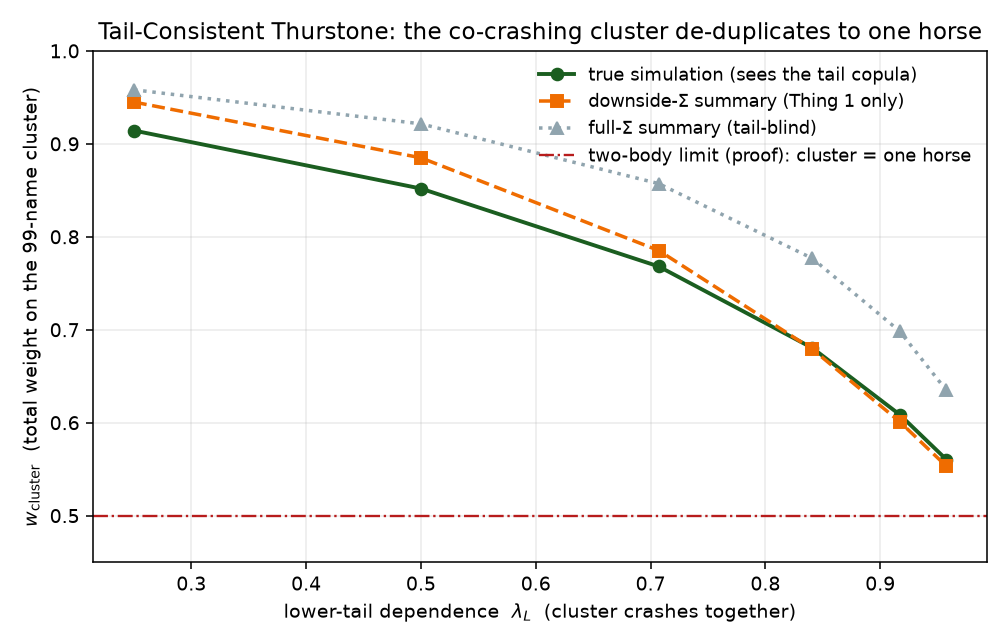
\includegraphics[width=0.80\textwidth]{figures/tail_consistency.png}
  \caption{Tail consistency. One independent asset versus a $99$-name cluster
  with Clayton lower-tail dependence $\lambda_L$ (assets crash together, rally
  independently; standard-normal margins; $M=1.5\times10^5$; loss-side race on
  centred performances). As $\lambda_L\to1$ the cluster's combined weight falls
  toward the two-body limit $\tfrac12$ (\Cref{prop:tail})---the $99$ names
  de-duplicate to a single horse. Driving the race by the downside semicovariance
  (lower partial co-moments) recovers almost all of the effect; the full
  covariance is tail-blind and stays far above. The small residual gap between the
  downside-covariance summary and the true tail copula is the part of the
  dependence that is not a second moment at all.}
  \label{fig:tail}
\end{figure}

\begin{remark}[Two layers of tail dependence]
\label{rem:twolayers}
Full covariance is blind to the downside asymmetry (\Cref{fig:tail}, grey); the
downside semicovariance captures the asymmetry but is still a second moment,
dominated by moderate losses; the exact object is the tail copula of
$\min_{i\in G}$, which the argmin reads directly from a tail-dependent simulation
and which no covariance summary represents. In the loss-side race the
second-moment shadow is a close approximation (\Cref{fig:tail}, orange versus
green), so a downside-covariance estimator suffices in practice, with the
simulation path as the exact limit.
\end{remark}

\begin{remark}[Centring]
\label{rem:centring}
The race must run on \emph{centred} performances. With non-zero means the extreme
order statistic tracks the lowest-drift asset and swamps the tail-dependence
signal; in the tilt the abilities carry the location and the race acts on the
centred residual.
\end{remark}

\subsection{The implied objective}
\label{sec:objective}

The tilt is defined procedurally, by winning probabilities. It is natural to ask
what objective, if any, it optimizes. It optimizes a recognizable one.

Write $\theta = -a$ (so larger $\theta$ denotes a stronger competitor, since the
minimum wins) and define the \emph{expected-best} potential
\begin{equation}
  G_C(\theta) = \E\Big[\max_i\,(\theta_i + \eta_i)\Big], \qquad
  \eta \sim \mathcal{N}(0, C).
  \label{eq:surplus}
\end{equation}

\begin{theorem}[Implied objective]
\label{thm:objective}
$G_C$ is convex and $C^\infty$ in $\theta$, the weights are its gradient,
$w = \nabla G_C(\theta)$, and equivalently $w$ is the unique solution of the
regularized program
\begin{equation}
  w \;=\; \argmaxop_{p \in \Delta}\ \big\{\, \langle \theta, p \rangle
  - \Omega_C(p) \,\big\},
  \label{eq:regularized}
\end{equation}
where $\Omega_C = G_C^{*}$ is a convex regularizer (the Fenchel conjugate of
$G_C$) supported on the simplex $\Delta$.
\end{theorem}
\begin{proof}
$G_C$ is an expectation of functions affine in $\theta$, hence convex; with an
almost-surely unique maximizer the envelope theorem gives
$\partial G_C/\partial\theta_i = \Prob(i = \argmaxop_k(\theta_k + \eta_k)) = w_i$,
i.e.\ $w = \nabla G_C$ (the Williams--Daly--Zachary identity
\parencite{williams1977, mcfadden1981}). Equation~\eqref{eq:regularized} is the
Fenchel--Young duality for the convex $G_C$.
\end{proof}

So the portfolio maximizes an ability-weighted exposure $\langle\theta,p\rangle$
minus a convex \emph{diversification penalty} $\Omega_C$ that is determined by
the correlation---a mean--(convex-risk) allocator whose feasible set is the
simplex, which is why the solution is long-only and fully invested. This is the
random-utility ``social-surplus'' / perturbed-optimizer construction
\parencite{mcfadden1981, williams1977, berthet2020}. The choice of perturbation
is decisive: Gumbel noise yields $\Omega = $ Shannon entropy and $w = $ softmax,
a \emph{correlation-blind} (Lucian) allocator; Gaussian noise with covariance
$C$ makes $\Omega_C$ \emph{correlation-aware}, which is precisely what produces
the redundancy consistency of \Cref{prop:redundancy}. Finally, since
$w = \nabla G_C(\theta)$ is the gradient of a convex potential, it is
automatically smooth---consistent with \Cref{thm:smooth}. (For general $C$ the
regularizer $\Omega_C$ has no closed form, unlike the entropy/softmax special
case, but it provably exists and is convex, which is all we use.)

\subsection{Any simulation, and the implied penalty}
\label{rem:anysim}

Nothing in \Cref{thm:objective} uses Gaussianity. For any centred performance law
$S$ set $G_S(\theta) = \E_{\eta\sim S}[\max_i(\theta_i + \eta_i)]$. This is convex
in $\theta$, so $w = \nabla G_S(\theta) =
\argmaxop_{p\in\Delta}\{\langle\theta, p\rangle - \Omega_S(p)\}$ with
$\Omega_S = G_S^{*}$ convex on the simplex. The weights always solve a
mean--(convex regularizer) program; the simulation enters only through the penalty
$\Omega_S$, which carries its full dependence, tails included.

This is the sense in which the portfolio is optimal for an arbitrary simulation.
It does not claim $\Omega_S$ is a \emph{named} risk measure: only the Gumbel
(Shannon entropy, softmax) and Gaussian (correlation-aware $\Omega_C$) cases are
closed-form, and in general $\Omega_S$ is implicit. Tail consistency
(\Cref{prop:tail}) is precisely the statement that $\Omega_S$ charges for tail
co-movement when $S$ carries it.

As the social-surplus conjugate, $\Omega_S$ is a \emph{generalized entropy}: it
rewards spreading across \emph{independent} options but counts only the
dependence-effective number of bets, so it will not reward spreading across
comonotone names (\Cref{prop:redundancy,prop:tail}). Locally it is quadratic, its
Hessian the \emph{inverse} of the winning-probability Jacobian on the simplex
tangent space (\Cref{sec:markowitz}), hence a Mahalanobis penalty in the choice
geometry. It is not a coherent risk measure (neither variance nor
CVaR), but the canonical Fenchel--Young regularizer of the perturbed argmax
\parencite{berthet2020}.

\subsection{Markowitz, reverse optimization, and the Thurstone inverse}
\label{sec:markowitz}

The implied objective of \Cref{thm:objective} is best read as a
reverse-optimization analogue of Markowitz. The comparison separates three roles
that are easily conflated: the benchmark, the return or ability vector that
rationalises it, and the risk or diversification geometry used to perturb it.

\paragraph{The Markowitz inverse.}
The long-only mean--variance problem
$w^M = \argmaxop_{p\in\Delta}\{\mu^\top p - \tfrac{\gamma}{2}p^\top\Sigma p\}$ has
first-order condition $\mu - \gamma\Sigma w^M - \lambda\mathbf 1 = 0$, that is
$w^M = \gamma^{-1}\Sigma^{-1}(\mu - \lambda\mathbf 1)$ (ignoring binding
inequalities). Expected returns are mapped to weights by the \emph{inverse}
covariance, and that inverse is the source of the method's fragility: a small
eigenvalue of $\Sigma$ becomes a large eigenvalue of $\Sigma^{-1}$, so a small
return component in a near-null direction can produce a large, unstable position.

\paragraph{Reverse optimization.}
Reverse (Black--Litterman / Grinold) optimization turns this around. If a benchmark
$w^0$ is optimal under a reference covariance $\Sigma_0$, it \emph{implies} the
return vector $\mu = \gamma\Sigma_0 w^0 + \lambda\mathbf 1$: the reverse problem
applies the covariance itself, not its inverse, inferring the linear reward that
would have made $w^0$ optimal under the reference geometry. Perturbing the
covariance to $\Sigma_\phi = \Sigma_0 + \phi\,\Delta\Sigma$ while holding $\mu$
fixed, and dropping constants and simplex-linear terms, gives the
\emph{benchmark-centered} program
\[
  w^M_\phi = \argminop_{p\in\Delta}\Big\{\tfrac{\gamma}{2}(p-w^0)^\top\Sigma_0(p-w^0)
  + \tfrac{\gamma\phi}{2}\,p^\top\Delta\Sigma\,p\Big\}.
\]
A covariance change poses no new optimization; it perturbs the benchmark. At
$\phi=0$ the solution is $w^0$, and for small $\phi$ it departs only as the added
penalty forces.

\paragraph{The Thurstone analogue.}
The tilt has the same structure, with the quadratic Markowitz geometry replaced by
the Fenchel geometry of the race. Calibration finds $\theta$ with
$w^0 = \nabla G_{S_0}(\theta)$, equivalently $\theta = \nabla\Omega_{S_0}(w^0)$ on
the simplex tangent space (up to the additive constant in $\theta$)---the analogue
of $\mu = \gamma\Sigma_0 w^0 + \lambda\mathbf 1$. Holding the score $\theta$ fixed
and tilting the law to $S_\phi$,
\[
  w^T_\phi = \argmaxop_{p\in\Delta}\{\theta^\top p - \Omega_{S_\phi}(p)\}
  = \argminop_{p\in\Delta}\{\Omega_{S_\phi}(p) - \nabla\Omega_{S_0}(w^0)^\top p\}.
\]
Adding and subtracting $\Omega_{S_0}(p)$ writes this as
\[
  w^T_\phi = \argminop_{p\in\Delta}\big\{ D_{\Omega_{S_0}}(p, w^0)
  + [\Omega_{S_\phi}(p) - \Omega_{S_0}(p)] \big\},
\]
with $D_{\Omega_{S_0}}(p,w^0) = \Omega_{S_0}(p) - \Omega_{S_0}(w^0)
- \nabla\Omega_{S_0}(w^0)^\top(p-w^0)$ the Bregman divergence of the reference
regularizer. For a smooth perturbation $\Omega_{S_\phi} = \Omega_{S_0}
+ \phi\,\dot\Omega_{\Delta S} + O(\phi^2)$, so
\[
  w^T_\phi \approx \argminop_{p\in\Delta}\big\{ D_{\Omega_{S_0}}(p, w^0)
  + \phi\,\dot\Omega_{\Delta S}(p) \big\},
\]
the exact analogue of the reverse-Markowitz perturbation under
$\tfrac{\gamma}{2}(p-w^0)^\top\Sigma_0(p-w^0) \leftrightarrow D_{\Omega_{S_0}}(p,w^0)$
and $\tfrac{\gamma}{2}p^\top\Delta\Sigma\,p \leftrightarrow \dot\Omega_{\Delta S}(p)$.
Markowitz measures displacement from the benchmark by a quadratic form in
$\Sigma_0$; the tilt measures it by the Bregman divergence of the reference race.

\paragraph{The displaced inverse.}
Locally the two are closer still. For $p = w^0 + \delta$,
$D_{\Omega_{S_0}}(w^0+\delta, w^0) = \tfrac12\delta^\top H_0\delta + O(\|\delta\|^3)$
with $H_0 = \nabla^2\Omega_{S_0}(w^0)$. Convex duality gives
$H_0 = [\nabla^2 G_{S_0}(\theta)]^{-1} = [\nabla_\theta w(\theta)]^{-1}$, the inverse
of the winning-probability Jacobian, so the local penalty is
$\tfrac12\delta^\top[\nabla_\theta w(\theta)]^{-1}\delta$: a Markowitz-like
quadratic with the \emph{inverse choice-sensitivity} in place of $\Sigma$. The
Markowitz inverse is not replicated but \emph{displaced}, from return space to
choice space---$\Sigma^{-1}$ maps returns to weights, whereas
$[\nabla_\theta w(\theta)]^{-1}$ maps weight displacements to ability costs. The
Fast Ability Transform is the global form of this inverse, from desired winning
probabilities to abilities under the reference race. The construction is therefore
inversion-free in the \emph{asset} covariance---it samples from the dependence law
and never forms $\Sigma^{-1}$---yet convex duality still leaves an inverse, now a
bounded, simplex-supported curvature rather than a lever on small covariance
eigenmodes. Singular dependence merely means some assets are effective duplicates
in the race, not that the optimizer takes explosive offsetting positions.

\paragraph{A selection identity.}
For the Gaussian workhorse one identity sits behind this local geometry. With
$X = \theta + \eta$, $\eta\sim\mathcal N(0,C)$, and $I = \argmaxop_k X_k$, the
weight is $w_i(\theta) = \Prob_\theta(I=i)$ and a selection form of Tweedie's
formula holds,
\[
  \E[X \mid I=i] = \theta + C\,\nabla_\theta\log w_i(\theta), \qquad
  \frac{\partial w_i}{\partial\theta_j}
  = w_i(\theta)\,\big[C^{-1}(\E[X\mid I=i] - \theta)\big]_j.
\]
The score of the winning probability is the conditional displacement of the latent
performance given that $i$ won; the Jacobian $\nabla_\theta w(\theta)$, whose
inverse is the local penalty curvature, is a matrix of selection sensitivities.
Tweedie's identity, the Markowitz analogy, and the Fenchel dual all point to the
same object: the local geometry of the winning-probability map.

\paragraph{Not a return forecast.}
None of this makes the tilt a return-forecasting method. The linear term $\theta$ is
benchmark-implied ability, not expected return; against a true $\mu$ the change in
expected return, $(w^T - w^0)^\top\mu$, need not be positive. The claim is
geometric: the tilt holds a benchmark anchor, infers the scores that rationalise it
under a reference race, and perturbs under a dependence-aware race. Its potential
benefit is a better diversification geometry---fewer duplicated bets, less tail
co-crash concentration, smoother turnover---while staying close to a return-bearing
benchmark. The relation to capitalization weighting is then that of \Cref{sec:capm}:
efficiency on a restricted universe depends on the whole $\Sigma_U^{-1}$, which
renormalised cap weights ignore, and the tilt recovers part of that
field-dependence without inversion, since assets redundant in the dependence law
compete in the race and their combined weight falls with their effective
distinctness. In one line: Markowitz is expected return minus a quadratic
covariance penalty; reverse Markowitz reads the benchmark as an implied return
perturbed by a covariance change; the tilt is benchmark-implied ability minus a
race-induced convex penalty; and locally that penalty is Markowitz's, with
$[\nabla_\theta w(\theta)]^{-1}$ replacing $\Sigma$.

\section{Smoothness and Turnover}
\label{sec:smoothness}

In the online (rebalancing) setting the correlation estimate moves slowly from
one period to the next, and we want the portfolio to move slowly with it:
turnover should track \emph{genuine} change in the correlation, not estimation
or sampling noise. We show the weight map is smooth, with a turnover bound, and
that a common-seed Monte-Carlo realisation inherits it.

Fix the abilities $a$ (calibrated once; they drift slowly) and view the weights
as a function of the correlation matrix $C$. Centring performances by $a$, asset
$i$ wins iff $Y = X - a \sim \mathcal{N}(0, C)$ lands in the \emph{fixed}
polyhedral cone
\begin{equation}
  A_i = \{\, y : y_i - y_j \le a_j - a_i \ \ \forall j \,\},
  \label{eq:wincone}
\end{equation}
so the weight is
$w_i(C) = \Prob_{Y\sim\mathcal{N}(0,C)}(Y\in A_i) = \int_{A_i}\varphi_C(y)\,dy$,
with $\varphi_C$ the $\mathcal{N}(0,C)$ density.

\begin{theorem}[Smoothness]
\label{thm:smooth}
On the open cone of positive-definite correlation matrices, $w_i(C)$ is
$C^\infty$ in $C$ (and in $a$). Moreover, on any compact subset whose smallest
eigenvalue is bounded below by $\lambda > 0$, the map is Lipschitz:
\begin{equation}
  \|w(C_1) - w(C_0)\|_1 \;\le\; L_\lambda \,\|C_1 - C_0\|,
  \qquad L_\lambda = O(1/\lambda).
  \label{eq:lip}
\end{equation}
\end{theorem}

\begin{proof}
The region $A_i$ in \eqref{eq:wincone} is independent of $C$. On the
positive-definite cone $\det C$ and $C^{-1}$ are real-analytic, so
$(C, y) \mapsto \varphi_C(y)$ is $C^\infty$ in $C$; its $C$-derivatives are
polynomials in $y$ times $\varphi_C(y)$, which are integrable and locally
dominated uniformly on compact sets. Differentiation under the integral sign
then gives $w_i \in C^\infty$. For the gradient, Price's theorem
\parencite{price1958}---the Gaussian identity
$\partial \varphi_C/\partial C_{jk} = \partial^2 \varphi_C/\partial y_j\,\partial y_k$
for $j \neq k$---followed by the divergence theorem over the cone $A_i$ rewrites
$\partial w_i/\partial C_{jk}$ as an integral of $\varphi_C$ over the boundary
faces of $A_i$ (the pairwise-tie hyperplanes), which is finite. The gradient is
therefore bounded; since the conditioning of $C$ controls the tie-boundary
density, the bound is $O(1/\lambda)$, giving \eqref{eq:lip}.
\end{proof}

The Lipschitz constant degrades as $C$ approaches singularity
($\lambda \to 0$)---the expected caveat that near-degenerate correlation makes
ties, and hence weights, sensitive. This motivates keeping $C$ well-conditioned
and regenerating the path ensemble when its effective sample size collapses.

\paragraph{Rank deficiency and conditioning.}
The square root is not the inversion it replaces, and the difference is what keeps
the method well posed where minimum variance is not. Inversion amplifies small
eigenvalues ($\lambda^{-1}\to\infty$), so a rank-deficient $\Sigma$ makes
$\Sigma^{-1}$ undefined; the root attenuates them ($\sqrt{\lambda}\to 0$), so a
rank-$r$ correlation merely yields draws supported on an $r$-dimensional subspace,
a valid degenerate race whose winning frequencies still lie on the simplex.
Moreover we only ever \emph{multiply} by $C^{1/2}$, never solve with it, and
$\operatorname{cond}(C^{1/2}) = \sqrt{\operatorname{cond}(C)}$, so ill-conditioning
does not propagate. What degrades near degeneracy is thus not the allocation but
the turnover bound: $C^{1/2}$ is continuous through coincident eigenvalues yet only
H\"older-$\tfrac12$ there ($\partial_\lambda\sqrt\lambda \sim \lambda^{-1/2}$),
which is the $O(1/\lambda)$ of \eqref{eq:lip}. The factor route of
\Cref{sec:computation} removes even this: with
$C = BB^\top + \operatorname{diag}(\psi)$ the idiosyncratic floor bounds
$\lambda_{\min}\ge\min_i\psi_i$, regularizing both the root and the Lipschitz
constant while never forming a dense $C^{1/2}$.\footnote{Rank deficiency is, if
anything, favourable for the estimate: it lowers the effective dimension of the
integrand, the regime in which quasi-Monte-Carlo excels. The eigenvalue (PCA) root
loads variance onto the leading components, so a randomized Sobol' sequence with
its best-equidistributed coordinates assigned to the factor directions---the PCA
construction familiar from quasi-Monte-Carlo pricing---integrates the race
accurately with far fewer paths.}

\paragraph{Common-seed transport.}
We realise $w(C)$ by Monte Carlo with a \emph{fixed} set of standard-normal
seeds $Z_1, \dots, Z_M$ and the symmetric square root $S(C) = C^{1/2}$ (itself
$C^\infty$ on the positive-definite cone): the paths are
$\widehat{Y}_m(C) = S(C)\,Z_m$ and
$\widehat{w}_i(C) = M^{-1}\sum_m \mathbf{1}[\widehat{Y}_m(C) \in A_i]$. Each
indicator is piecewise constant in $C$, flipping only when a path crosses a face
of $A_i$. A step $\Delta C$ thus moves the realized weights by two contributions:
the systematic response $O(\|\Delta C\|)$ inherited from \Cref{thm:smooth}, and a
sampling term from the $O(M\,\|\Delta C\|)$ boundary crossings, which net out
stochastically to $O(\sqrt{\|\Delta C\|/M})$. Common seeds are what keep the second
small: when $\Delta C = 0$ the same seeds give the same winners and
$\Delta\widehat{w} = 0$ \emph{exactly}, whereas fresh resampling carries an
$O(1/\sqrt{M})$ floor whether or not $C$ moved. The sampling offset cancels in
differences, leaving only the (smaller) crossing term, which shrinks with the path
budget $M$; this is the mechanism behind the incremental (online) update. The
realized turnover is therefore not zero at finite $M$ but is far below fresh
resampling and vanishes with the path budget. (Quasi-Monte-Carlo sharpens the
\emph{level} of each $\widehat{w}(C)$, but not this difference, whose noise is set
by the moved decision boundary rather than by integration error.)

\Cref{tab:turnover} confirms both statements numerically along a $60$-step
convex path between two random correlation matrices.

\begin{table}[h]
  \centering
  \caption{Turnover along a $60$-step correlation path ($n = 8$,
  $M = 4\times10^4$). Common-seed transport tracks genuine correlation change;
  fresh resampling carries a noise floor that does not vanish when the
  correlation is held static.}
  \label{tab:turnover}
  \begin{tabular}{lc}
    \toprule
    Quantity & Value \\
    \midrule
    mean $\|\Delta C\|_1$ per step                          & $0.372$ \\
    mean $\|\Delta w\|_1$, common-seed transport            & $0.0043$ \\
    mean $\|\Delta w\|_1$, fresh resampling                 & $0.0145$ \\
    Lipschitz ratio $\|\Delta w\|_1 / \|\Delta C\|_1$ (max) & $0.027$ \\
    static $\Delta C = 0$: transport                        & $0$ (exact) \\
    static $\Delta C = 0$: resampling                       & $0.0157$ \\
    \bottomrule
  \end{tabular}
\end{table}

